\documentclass{article}
\usepackage{amsmath}
\usepackage{geometry}
\usepackage{graphicx}
\usepackage{hyperref}
\usepackage{listings}
\usepackage{minted} % For better code highlighting if available, otherwise listings
\usepackage{tikz} % Added for TikZ figures
\usetikzlibrary{shapes.geometric, positioning, arrows.meta} % Added TikZ libraries and arrows.meta

\geometry{a4paper, margin=1in}

\title{Quantum Dot Simulation Suite Documentation}
\author{AI Software Developer}
\date{\today}

\begin{document}
\maketitle
\tableofcontents
\newpage

\section{Introduction}
This document provides an overview of the physics and code structure for a suite of quantum dot simulators. These simulators solve the Schrödinger and Poisson equations self-consistently to model the behavior of electrons in semiconductor quantum dot devices. The suite includes tools for 1D and 2D simulations, as well as specialized simulations for pinch-off characteristics, charge stability diagrams, and Coulomb diamonds. The simulations are designed to mimic experiments performed on gated semiconductor nanostructures.

\section{Semiconductor Quantum Dot Devices}
Semiconductor quantum dots (QDs) are nanoscale structures capable of confining electrons (or holes) in all three spatial dimensions. Due to this strong confinement, their energy levels become discrete, similar to those of an atom, leading to them often being referred to as "artificial atoms".

\subsection{Formation in Semiconductor Heterostructures}
A common method for creating QDs is by using patterned metallic gates on the surface of a semiconductor heterostructure. A typical structure involves growing a layer of a wider bandgap semiconductor (like AlGaAs) on top of a narrower bandgap semiconductor (like GaAs). Electrons from donor atoms in the AlGaAs layer transfer to the GaAs, forming a thin layer of highly mobile electrons at the interface, known as a two-dimensional electron gas (2DEG). This 2DEG is confined in the growth direction (typically z) by the bandgap difference.

Metallic gates deposited on the surface above the 2DEG can deplete the underlying electron gas when a negative voltage is applied. By carefully designing the shape and voltage of multiple gates, the 2DEG can be locally depleted, pinching off channels and isolating small puddles of electrons. These isolated puddles form the quantum dots, confined laterally (in x and y) by the electrostatic potential created by the gates.

Figure \ref{fig:cross_section} illustrates a schematic cross-section of such a device structure.

\begin{figure}[h!]
    \centering
    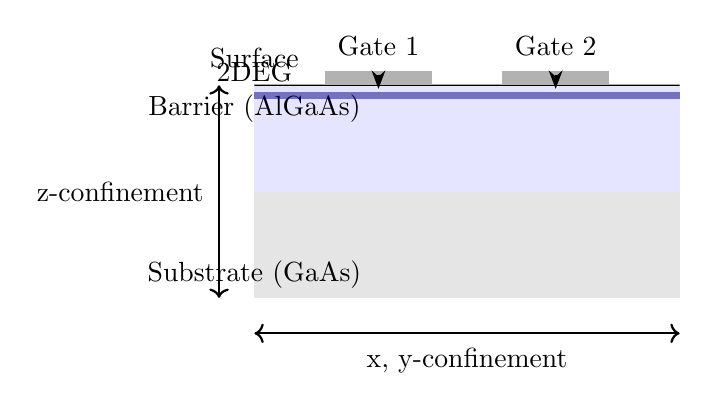
\begin{tikzpicture}[scale=0.9, node distance=0.5cm]
        % Define layers
        \coordinate (origin) at (0,0);
        \fill[gray!20] (origin) rectangle (6,-1.5); % Substrate
        \node[below=0.75cm of origin, text centered] (substrate_label) {Substrate (GaAs)};

        \coordinate (barrier_bottom) at (0,0);
        \fill[blue!10] (barrier_bottom) rectangle (6,1.5); % Barrier
        \node[above=0.75cm of barrier_bottom, text centered] (barrier_label) {Barrier (AlGaAs)};

        % 2DEG layer - represent as a thin shaded region
        \coordinate (2deg_bottom) at (0,1.3);
        \fill[blue!50!black, opacity=0.5] (2deg_bottom) rectangle (6,1.4);
        \node[above=0.1cm of 2deg_bottom, text centered] (2deg_label) {2DEG};

        % Surface
        \coordinate (surface) at (0,1.5);
        \draw (surface) -- (6,1.5);
        \node[above=0.1cm of surface, text centered] (surface_label) {Surface};

        % Gates on the surface
        \fill[black!30] (1,1.5) rectangle (2.5,1.7);
        \node[above=2pt] at (1.75,1.7) {Gate 1};
        \fill[black!30] (3.5,1.5) rectangle (5,1.7);
        \node[above=2pt] at (4.25,1.7) {Gate 2};

        % Indicate potential influence with dashed arrows
        \draw[->, dashed, thick, >=Stealth] (1.75,1.65) -- (1.75,1.45);
        \draw[->, dashed, thick, >=Stealth] (4.25,1.65) -- (4.25,1.45);

        % Add labels for confinement directions
        \draw[<->, thick] (-0.5,-1.5) -- (-0.5,1.5);
        \node[left=2pt of {-0.5,0}] {z-confinement};

        \draw[<->, thick] (0,-2) -- (6,-2);
        \node[below=2pt of {3,-2}] {x, y-confinement};
    \end{tikzpicture}
    \caption{Schematic cross-section of a gated semiconductor quantum dot device. Top gates deplete the 2DEG, creating lateral confinement.}
    \label{fig:cross_section}
\end{figure}

\subsection{Key Properties: Confinement and Coulomb Blockade}
The strong confinement in QDs leads to several key properties:
\begin{itemize}
    \item \textbf{Quantum Confinement}: The energy levels for electrons in the dot become discrete, separated by energy gaps much larger than the thermal energy at low temperatures. Electrons can only occupy these specific energy states.
    \item \textbf{Coulomb Blockade}: Adding an extra electron to a quantum dot requires overcoming the electrostatic repulsion from the electrons already present. This costs an additional energy, the charging energy ($E_C$). This energy cost leads to a "Coulomb blockade" of current flow when the dot is connected to leads, unless the applied voltage is sufficient to overcome $E_C$.
\end{itemize}
These properties make QDs promising candidates for qubits in quantum computing and for studying fundamental quantum mechanics.

\subsection{Simulated Device Geometry: Double Quantum Dot}
The simulation suite focuses on a common and important device structure: the double quantum dot (DQD). A DQD consists of two quantum dots coupled together, typically formed by an arrangement of plunger gates (P1, P2) that define the potential wells for each dot, and barrier gates (B1, B2, B3) that control the coupling between the dots and to external leads (not explicitly simulated here, but implied).

The scripts model the gates using 2D (or 1D in \texttt{simulate\_1d\_dot.py}) Gaussian potential profiles, where the amplitude is proportional to the applied gate voltage. This provides a smooth, realistic potential landscape. Figure \ref{fig:gate_layout} shows a top-down schematic of the gate layout used in the 2D simulations.

\begin{figure}[h!]
    \centering
    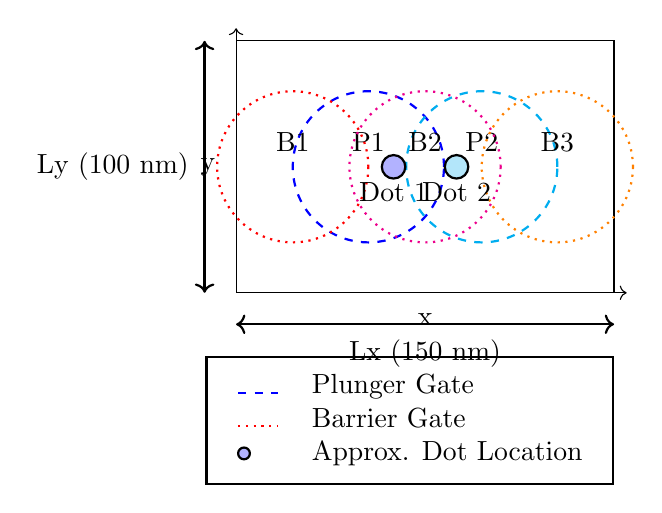
\begin{tikzpicture}[scale=0.8]
        % Simulation domain boundary
        \draw (0,0) rectangle (6,4);
        % Remove coordinate labels
        % node[below left] at (0,0) {};
        % node[above right] at (6,4) {};

        % Add axis labels, slightly further out
        \node[below=4pt] at (3,0) {x};
        \node[left=4pt] at (0,2) {y};
        \draw[->] (0,0) -- (6.2,0); % x-axis arrow
        \draw[->] (0,0) -- (0,4.2); % y-axis arrow


        % Gate positions (scaled from simulation parameters)
        % Lx=150e-9, Ly=100e-9. Scale factor: 25 nm/unit.
        % P1: (52.5, 50) nm -> (2.1, 2.0)
        % P2: (97.5, 50) nm -> (3.9, 2.0)
        % B1: (22.5, 50) nm -> (0.9, 2.0)
        % B2: (75, 50) nm -> (3.0, 2.0)
        % B3: (127.5, 50) nm -> (5.1, 2.0)
        % Gate std dev vis ~ 20nm. Let's use a visual radius of 30nm = 1.2 units.

        % Gate Ellipses (center, x-radius, y-radius)
        % Plungers (P1, P2) - typically negative voltage, create wells
        \draw[blue, dashed, thick] (2.1, 2.0) ellipse (1.2 and 1.2); \node[above=2pt] at (2.1, 2.0) {P1};
        \draw[cyan, dashed, thick] (3.9, 2.0) ellipse (1.2 and 1.2); \node[above=2pt] at (3.9, 2.0) {P2};

        % Barriers (B1, B2, B3) - typically positive voltage, create barriers
        \draw[red, dotted, thick] (0.9, 2.0) ellipse (1.2 and 1.2); \node[above=2pt] at (0.9, 2.0) {B1};
        \draw[magenta, dotted, thick] (3.0, 2.0) ellipse (1.2 and 1.2); \node[above=2pt] at (3.0, 2.0) {B2};
        \draw[orange, dotted, thick] (5.1, 2.0) ellipse (1.2 and 1.2); \node[above=2pt] at (5.1, 2.0) {B3};

        % Indicate approximate dot locations (potential minima)
        % Use slightly larger nodes for visibility, adjust positioning
        \node[draw, circle, inner sep=3pt, fill=blue!30, thick] at (2.5, 2.0) {}; \node[below=2pt] at (2.5, 2.0) {Dot 1};
        \node[draw, circle, inner sep=3pt, fill=cyan!30, thick] at (3.5, 2.0) {}; \node[below=2pt] at (3.5, 2.0) {Dot 2};

        % Add scale bar
        \draw[<->, thick] (0, -0.5) -- (6, -0.5) node[midway, below=2pt] {Lx (150 nm)};
        \draw[<->, thick] (-0.5, 0) -- (-0.5, 4) node[midway, left=2pt] {Ly (100 nm)};

        % Add a simple legend, position it clearly outside the main box
        \node[below right, inner sep=5pt, draw, thick, anchor=north east] at (6,-1) { % Adjusted position and anchor
            \begin{tabular}{ll}
                \tikz{\draw[blue, dashed, thick] (0,0) -- (0.5,0);} & Plunger Gate \\
                \tikz{\draw[red, dotted, thick] (0,0) -- (0.5,0);} & Barrier Gate \\
                \tikz{\node[draw, circle, inner sep=1.5pt, fill=blue!30, thick] {};} & Approx. Dot Location \\ % Match node size
            \end{tabular}
        };

    \end{tikzpicture}
    \caption{Top-down schematic of the gate layout for the simulated double quantum dot. Plunger gates (P1, P2) define the dots, while barrier gates (B1, B2, B3) control coupling.}
    \label{fig:gate_layout}
\end{figure}

By simulating the electronic properties of this DQD structure under varying gate voltages, the suite can reproduce characteristic experimental results like pinch-off curves and charge stability diagrams.

\section{Physics Background}
The core of the simulation lies in the self-consistent solution of the Schrödinger and Poisson equations.

\subsection{Schrödinger Equation}
The time-independent Schrödinger equation describes the quantum mechanical states of electrons in a given potential. For a single electron with effective mass $m_{\text{eff}}$ in a potential $V(\mathbf{r})$, the equation is:
\begin{equation}
    \left[ -\frac{\hbar^2}{2m_{\text{eff}}} \nabla^2 + V(\mathbf{r}) \right] \psi_i(\mathbf{r}) = E_i \psi_i(\mathbf{r})
\end{equation}
where $\hbar$ is the reduced Planck constant, $\psi_i(\mathbf{r})$ are the eigenfunctions (wavefunctions), and $E_i$ are the corresponding eigenvalues (energy levels). The total potential $V(\mathbf{r})$ is a sum of the external potential $V_{\text{ext}}(\mathbf{r})$ (due to gates, as discussed in Section 2) and the electrostatic potential $\phi(\mathbf{r})$ due to the electron charge itself: $V(\mathbf{r}) = V_{\text{ext}}(\mathbf{r}) - e \phi(\mathbf{r})$.

\subsection{Poisson Equation}
The Poisson equation relates the electrostatic potential $\phi(\mathbf{r})$ to the charge density $\rho(\mathbf{r})$:
\begin{equation}
    \nabla^2 \phi(\mathbf{r}) = -\frac{\rho(\mathbf{r})}{\epsilon}
\end{equation}
where $\epsilon = \epsilon_r \epsilon_0$ is the permittivity of the material ($\epsilon_r$ is the relative permittivity and $\epsilon_0$ is the vacuum permittivity). The charge density $\rho(\mathbf{r})$ is calculated from the occupied electron states:
\begin{equation}
    \rho(\mathbf{r}) = -e \sum_i f(E_i, E_F, T) |\psi_i(\mathbf{r})|^2
\end{equation}
where $e$ is the elementary charge, and $f(E_i, E_F, T)$ is the Fermi-Dirac distribution function, which gives the probability of occupation for an energy state $E_i$ at a given Fermi level $E_F$ and temperature $T$. A factor of 2 is included for spin degeneracy. In the current implementation, a zero-temperature approximation ($T \to 0$) is often used, where $f(E_i, E_F, 0) = 1$ if $E_i < E_F$ and $0$ otherwise.

\subsection{Self-Consistent Solution}
The Schrödinger and Poisson equations are coupled: the potential in the Schrödinger equation depends on the charge density (via the Poisson equation), and the charge density in the Poisson equation depends on the wavefunctions (via the Schrödinger equation). This necessitates a self-consistent solution:
\begin{enumerate}
    \item \textbf{Initial Guess}: Start with an initial guess for the electrostatic potential $\phi(\mathbf{r})$ (e.g., $\phi(\mathbf{r}) = 0$ or the converged potential from a nearby gate voltage point for sweep simulations).
    \item \textbf{Total Potential}: Calculate the total potential $V(\mathbf{r}) = V_{\text{ext}}(\mathbf{r}) - e \phi(\mathbf{r})$.
    \item \textbf{Solve Schrödinger Equation}: Solve the Schrödinger equation using $V(\mathbf{r})$ to find eigenvalues $E_i$ and eigenvectors $\psi_i(\mathbf{r})$.
    \item \textbf{Calculate Charge Density}: Calculate the new charge density $\rho_{\text{new}}(\mathbf{r})$ using the computed $E_i$ and $\psi_i(\mathbf{r})$ and the Fermi-Dirac distribution.
    \item \textbf{Solve Poisson Equation}: Solve the Poisson equation with $\rho_{\text{new}}(\mathbf{r})$ to obtain a new electrostatic potential $\phi_{\text{new}}(\mathbf{r})$.
    \item \textbf{Check Convergence}: Compare $\phi_{\text{new}}(\mathbf{r})$ with the previous $\phi(\mathbf{r})$. If the difference (e.g., measured by a norm) is below a specified tolerance, the solution is converged.
    \item \textbf{Mix and Iterate}: If not converged, mix the new and old potentials (e.g., $\phi(\mathbf{r}) = (1-\alpha)\phi(\mathbf{r}) + \alpha\phi_{\text{new}}(\mathbf{r})$, where $\alpha$ is a mixing parameter, typically between 0 and 1) and return to step 2. Mixing is crucial for numerical stability. Adaptive mixing schemes can also be employed.
\end{enumerate}
This iterative process is repeated until convergence is achieved or a maximum number of iterations is reached.

\section{Code Documentation}
The simulation suite consists of several Python scripts, each tailored for specific types of simulations. They share common physical constants, material parameters, and core solver functions.

\subsection{Common Elements}
\subsubsection{Physical Constants and Material Parameters}
All scripts define:
\begin{itemize}
    \item \textbf{Physical Constants}: $\hbar$ (hbar), $m_e$ (electron mass), $e$ (elementary charge), $\epsilon_0$ (vacuum permittivity).
    \item \textbf{Material Parameters (GaAs)}: $m_{\text{eff}}$ (effective mass, $0.067 \cdot m_e$), $\epsilon_r$ (relative permittivity, $12.9$).
\end{itemize}

\subsubsection{Simulation Grid}
A 1D or 2D numerical grid is defined:
\begin{itemize}
    \item \texttt{L} (1D) or \texttt{Lx}, \texttt{Ly} (2D): Length of the simulation domain.
    \item \texttt{N} (1D) or \texttt{Nx}, \texttt{Ny} (2D): Number of grid points.
    \item \texttt{x}, \texttt{y}: Arrays of grid point coordinates.
    \item \texttt{dx}, \texttt{dy}: Grid spacing.
\end{itemize}
For 2D simulations, \texttt{X} and \texttt{Y} meshgrids are created using \texttt{np.meshgrid} with \texttt{indexing='ij'} to match matrix indexing conventions.

\subsubsection{Core Functions}
\begin{description}
    \item[\texttt{get\_external\_potential(X, Y, voltages)}] Calculates the external potential profile based on gate voltages. Uses Gaussian profiles for each gate's influence, as described in Section 2.3. The \texttt{voltages} argument is a dictionary mapping gate names (e.g., "P1", "B2") to their applied voltage values.
    \item[\texttt{solve\_schrodinger(potential)}] (1D) or \texttt{solve\_schrodinger\_2d(potential\_2d)}] Solves the time-independent Schrödinger equation using a finite difference method on a sparse matrix representation of the Hamiltonian. It finds the lowest few eigenvalues and corresponding eigenvectors using \texttt{scipy.sparse.linalg.eigsh}.
    \item[\texttt{calculate\_charge\_density(eigenvalues, eigenvectors, fermi\_level)}] (1D) or \texttt{calculate\_charge\_density\_2d(eigenvalues, eigenvectors\_2d, fermi\_level)}] Calculates the electron charge density using the computed eigenvalues, eigenvectors, and the specified Fermi level, applying the Fermi-Dirac distribution (often in the zero-temperature limit).
    \item[\texttt{solve\_poisson(charge\_density)}] (1D) or \texttt{solve\_poisson\_2d(charge\_density\_2d)}] Solves the Poisson equation using a finite difference method with Dirichlet boundary conditions (potential fixed at boundaries, typically to zero). It constructs a sparse matrix for the Laplacian operator and solves the linear system using \texttt{scipy.sparse.linalg.spsolve} or an iterative solver like GMRES as a fallback.
    \item[\texttt{solve\_poisson\_2d\_spectral(charge\_density\_2d)}] (2D only) An alternative Poisson solver using spectral methods (Fast Fourier Transforms - FFTs). This method is efficient but inherently assumes periodic boundary conditions, which may not be physically appropriate for all device simulations compared to Dirichlet conditions.
    \item[\texttt{self\_consistent\_solver(voltages, fermi\_level, ...)}] (1D) or \texttt{self\_consistent\_solver\_2d(voltages, fermi\_level, ...)}] Implements the self-consistent iteration loop described in Section 3.3. It takes applied gate voltages and the Fermi level as input and iteratively calls the Schrödinger and Poisson solvers, mixing the potential until convergence is reached. It returns the converged total potential, charge density, eigenvalues, and eigenvectors (or None if convergence fails). The 2D version allows selecting the Poisson solver type.
\end{description}

\subsection{\texttt{simulate\_1d\_dot.py}}
This script performs a 1D Schrödinger-Poisson simulation for a quantum dot device.
\begin{itemize}
    \item \textbf{Purpose}: Simulates a 1D quantum dot, typically representing a cross-section or a simplified model of a double dot structure defined by plunger and barrier gates.
    \item \textbf{Key Features}:
        \begin{itemize}
            \item Defines a 1D grid.
            \item \texttt{get\_external\_potential}: Models gates using 1D Gaussian potentials.
            \item Solves 1D Schrödinger and Poisson equations.
            \item Performs self-consistent calculation.
            \item Plots potential profiles, charge density, and wavefunctions.
        \end{itemize}
\end{itemize}

\subsection{\texttt{simulate\_2d\_dot.py}}
This script performs a standard 2D Schrödinger-Poisson simulation for a fixed set of gate voltages.
\begin{itemize}
    \item \textbf{Purpose}: Simulates a 2D quantum dot, allowing for more realistic device geometries and potential landscapes. It's useful for visualizing the electron distribution and energy levels for a specific gate configuration.
    \item \textbf{Key Features}:
        \begin{itemize}
            \item Defines a 2D grid (\texttt{Nx}, \texttt{Ny}).
            \item \texttt{get\_external\_potential}: Models gates using 2D Gaussian potentials.
            \item \texttt{solve\_schrodinger\_2d}: Solves the 2D Schrödinger equation using a 5-point finite difference stencil.
            \item \texttt{solve\_poisson\_2d}: Solves the 2D Poisson equation using finite differences with Dirichlet boundary conditions.
            \item \texttt{solve\_poisson\_2d\_spectral}: An alternative spectral Poisson solver is available but not used by default in the main execution block.
            \item \texttt{self\_consistent\_solver\_2d}: Manages the 2D self-consistent loop. Allows selection of Poisson solver type.
            \item Plots 2D contour maps of total potential, external potential, charge density, and the ground state probability density. Includes visualization of gate positions as ellipses.
        \end{itemize}
\end{itemize}

\subsection{\texttt{simulate\_pinchoff.py}}
This script simulates the pinch-off characteristics of a quantum dot device by sweeping a gate voltage.
\begin{itemize}
    \item \textbf{Purpose}: To observe how the potential barrier under a gate changes as its voltage is swept, leading to channel pinch-off and depletion of electrons from the dot.
    \item \textbf{Key Features}:
        \begin{itemize}
            \item Based on the 2D simulation framework.
            \item Sweeps the voltage of a specified gate (e.g., "B2") over a defined range.
            \item For each voltage point in the sweep:
                \begin{itemize}
                    \item Runs the 2D self-consistent solver.
                    \item Estimates the minimum potential under the swept gate (barrier height) by sampling a slice of the potential.
                    \item Calculates the total number of electrons in the simulation domain by integrating the charge density.
                \end{itemize}
            \item Plots:
                \begin{itemize}
                    \item Pinch-off curve: Minimum barrier potential vs. swept gate voltage.
                    \item Number of electrons vs. swept gate voltage.
                    \item Final potential landscape for the last voltage point simulated.
                \end{itemize}
            \item Allows selection between finite difference and spectral Poisson solvers for the self-consistent loop.
        \end{itemize}
\end{itemize}

\subsection{\texttt{simulate\_charge\_stability.py}}
This script simulates charge stability diagrams by sweeping two gate voltages.
\begin{itemize}
    \item \textbf{Purpose}: To map out regions of stable integer electron numbers in the quantum dot system as two plunger gate voltages are varied. This reveals the characteristic honeycomb pattern of charge stability, a signature of Coulomb blockade.
    \item \textbf{Key Features}:
        \begin{itemize}
            \item Based on the 2D simulation framework, often with a reduced grid size (\texttt{Nx}, \texttt{Ny}) compared to \texttt{simulate\_2d\_dot.py} for faster computation over many voltage points.
            \item Sweeps two specified gate voltages (e.g., "P1", "P2") over 2D ranges.
            \item For each pair of (V\textsubscript{Gate1}, V\textsubscript{Gate2}) values:
                \begin{itemize}
                    \item Runs the 2D self-consistent solver.
                    \item Calculates the total number of electrons in the system by integrating the charge density using \texttt{calculate\_total\_electrons}.
                \end{itemize}
            \item Implements sweep strategies:
                \begin{itemize}
                    \item \texttt{row\_by\_row}: Standard raster scan.
                    \item \texttt{hilbert}: Sweeps points along a Hilbert space-filling curve using the \texttt{hilbertcurve} library. This strategy can improve convergence by using the converged potential from a nearby point in parameter space as a warm start (\texttt{initial\_potential\_V}) for the current point's self-consistent calculation. The \texttt{get\_hilbert\_order} function generates this sequence.
                \end{itemize}
            \item Stores the converged electrostatic potential from the previous point (in the chosen sweep order) to use as an initial guess (warm start) for the next point, potentially speeding up convergence, especially for the Hilbert sweep.
            \item Stores the total number of electrons for each voltage pair in a 2D map.
            \item Plots:
                \begin{itemize}
                    \item A 2D color map of the total number of electrons as a function of the two swept gate voltages.
                    \item An additional plot with rounded electron numbers to emphasize the integer plateaus and transitions.
                \end{itemize}
            \item Saves the raw data (voltages, electron map) to a `.npz` file and plots to image files in an output directory.
            \item Allows selection between finite difference and spectral Poisson solvers.
        \end{itemize}
\end{itemize}

\subsection{\texttt{simulate\_coulomb\_diamonds.py}}
This script simulates Coulomb diamonds, which are closely related to charge stability diagrams.
\begin{itemize}
    \item \textbf{Purpose}: Similar to charge stability, this script maps out electron number as a function of two gate voltages, typically used to identify Coulomb blockade regions and extract parameters like charging energy.
    \item \textbf{Key Features}:
        \begin{itemize}
            \item Based on the 2D simulation framework.
            \item Sweeps two specified gate voltages (e.g., "P1", "P2").
            \item For each voltage pair, runs the self-consistent solver and calculates the total number of electrons.
            \item Plots a 2D color map of the electron number, forming the characteristic Coulomb diamond pattern.
            \item Uses a zero-temperature approximation for charge density calculation.
            \item Note: This script is a simplified version compared to \texttt{simulate\_charge\_stability.py} and does not include features like warm starts or different sweep strategies.
        \end{itemize}
\end{itemize}

\section{Numerical Methods}
\subsection{Finite Difference Method}
The Schrödinger and Poisson equations are discretized using the finite difference method. For example, the second derivative $\frac{d^2\psi}{dx^2}$ is approximated as:
\begin{equation}
    \frac{d^2\psi}{dx^2} \approx \frac{\psi_{i+1} - 2\psi_i + \psi_{i-1}}{dx^2}
\end{equation}
where $\psi_i$ is the value of $\psi$ at grid point $x_i$, and $dx$ is the grid spacing. In 2D, the Laplacian $\nabla^2 = \frac{\partial^2}{\partial x^2} + \frac{\partial^2}{\partial y^2}$ is approximated using a 5-point stencil. This transforms the differential equations into a system of linear algebraic equations, which can be represented by sparse matrices.

\subsection{Eigenvalue Solvers}
The discretized Schrödinger equation becomes a matrix eigenvalue problem $H\psi = E\psi$. Sparse eigenvalue solvers from \texttt{scipy.sparse.linalg} (specifically \texttt{eigsh} for Hermitian matrices) are used to find the lowest energy eigenvalues and corresponding eigenvectors efficiently.

\subsection{Linear System Solvers}
The discretized Poisson equation becomes a linear system $A\phi = b$. Sparse linear solvers from \texttt{scipy.sparse.linalg} (specifically \texttt{spsolve} for direct solution or iterative solvers like GMRES (\texttt{gmres}) or LGMRES (\texttt{lgmres}) as fallbacks) are used to find the potential $\phi$. Dirichlet boundary conditions are implemented by modifying the corresponding rows and right-hand side vector of the linear system matrix.

\subsection{Spectral Method (Poisson)}
The \texttt{solve\_poisson\_2d\_spectral} function uses Fast Fourier Transforms (FFTs) to solve the Poisson equation in k-space. The equation $\nabla^2 \phi = -\rho/\epsilon$ becomes $-K^2 \Phi_k = -P_k/\epsilon$ in Fourier space, where $K^2 = k_x^2 + k_y^2$, and $\Phi_k, P_k$ are the Fourier transforms of $\phi, \rho$. This method is efficient for uniform grids and periodic boundary conditions. The DC component ($K=0$) is handled separately by setting $\Phi_k(0,0)=0$, which corresponds to setting the average potential to zero.

\section{Benchmark Results and Numerical Schemes}

\subsection{Benchmark Summary}

The performance of different numerical schemes for solving the Schrödinger-Poisson equations was benchmarked using the \texttt{benchmark\_solver\_schemes.py} script. The script tests different Poisson solvers (Finite Difference, Spectral) and Schrödinger solvers (various configurations of \texttt{eigsh} and \texttt{lobpcg}) under different scenarios, including cold starts with random voltages and warm starts with perturbed voltages.

Figure \ref{fig:benchmark_summary} shows a summary of the benchmark results across all scenarios. The plot illustrates the average total time, average Schrödinger solver time per iteration, and average Poisson solver time per iteration for each combination of solvers and scenarios. The number of converged samples out of the total number of samples is also indicated on the plot.

\begin{figure}[h!]
    \centering
    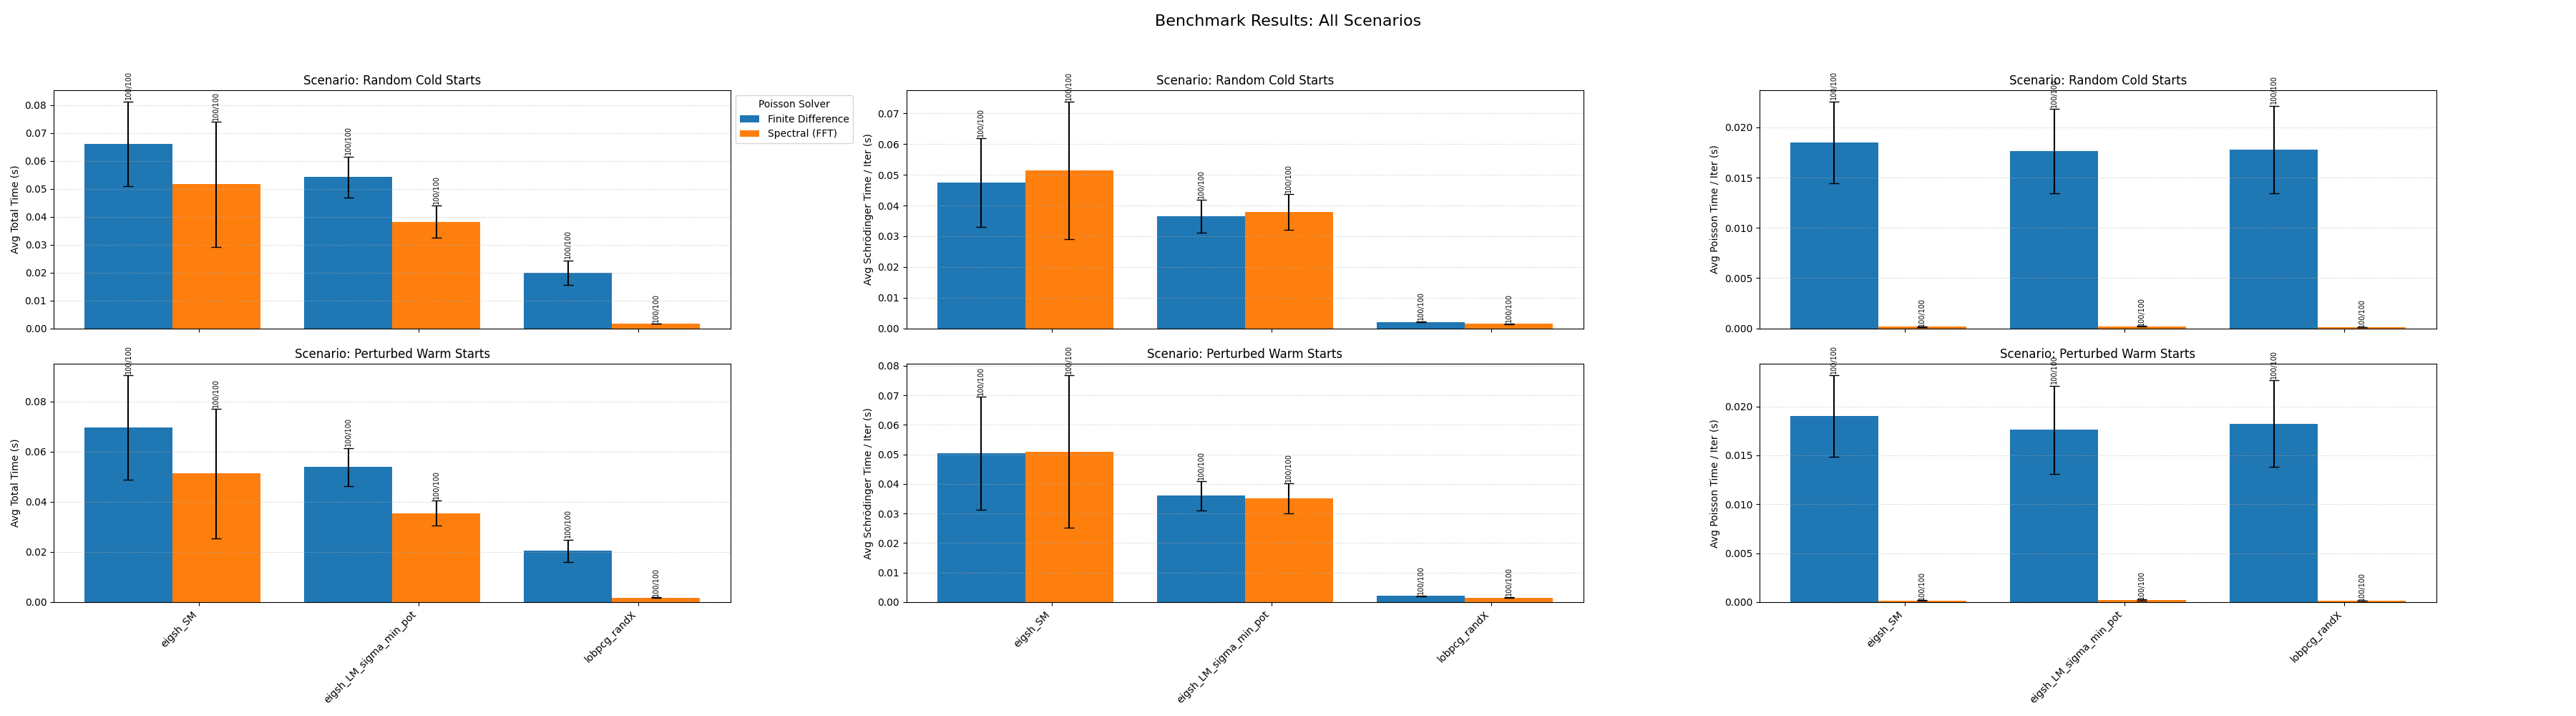
\includegraphics[width=\textwidth]{benchmark_summary_all_scenarios.png}
    \caption{Benchmark results for different Schrödinger-Poisson solver schemes across various scenarios. The plot shows the average total time, average Schrödinger solver time per iteration, and average Poisson solver time per iteration. The number of converged samples is also indicated.}
    \label{fig:benchmark_summary}
\end{figure}

\subsection{Numerical Schemes: Background and Implementation Details}

The simulation suite employs several numerical schemes to solve the Schrödinger and Poisson equations. This section provides a brief overview of these schemes, including their background and implementation details.

\subsubsection{Schrödinger Solvers}

\paragraph{Finite Difference Method}
The Schrödinger equation is discretized using the finite difference method (FDM). The second derivative is approximated using a central difference scheme:

\[
\frac{d^2\psi}{dx^2} \approx \frac{\psi_{i+1} - 2\psi_i + \psi_{i-1}}{dx^2}
\]

In 2D, the Laplacian is approximated using a 5-point stencil. This discretization transforms the Schrödinger equation into a sparse matrix eigenvalue problem.

\paragraph{\texttt{eigsh} (ARPACK)}
The \texttt{eigsh} function from \texttt{scipy.sparse.linalg} is used to solve the sparse matrix eigenvalue problem arising from the discretized Schrödinger equation. \texttt{eigsh} is a wrapper around the ARPACK library, which implements the Implicitly Restarted Arnoldi Method (IRAM).

ARPACK is designed for finding a few eigenvalues and eigenvectors of large sparse matrices. It is particularly efficient for finding eigenvalues at the extreme ends of the spectrum (i.e., smallest or largest magnitude).

Key parameters for \texttt{eigsh} include:
\begin{itemize}
    \item \texttt{k}: The number of eigenvalues and eigenvectors to find.
    \item \texttt{which}: Specifies which eigenvalues to find (e.g., \texttt{'SM'} for smallest magnitude, \texttt{'LM'} for largest magnitude).
    \item \texttt{sigma}: Specifies a shift value for finding eigenvalues near a particular value. Using \texttt{sigma} can improve convergence for interior eigenvalues.
    \item \texttt{tol}: The desired relative accuracy for the eigenvalues.
    \item \texttt{maxiter}: The maximum number of iterations allowed.
\end{itemize}

\paragraph{\texttt{lobpcg}}
The \texttt{lobpcg} function from \texttt{scipy.sparse.linalg} implements the Locally Optimal Block Preconditioned Conjugate Gradient (LOBPCG) method. LOBPCG is an iterative method for finding the lowest (or highest) eigenvalues and corresponding eigenvectors of a symmetric (or Hermitian) matrix.

LOBPCG is a block Krylov subspace method, which means it operates on a block of vectors simultaneously. This can lead to faster convergence compared to single-vector methods like the power method or the Lanczos method.

Key parameters for \texttt{lobpcg} include:
\begin{itemize}
    \item \texttt{X}: An initial guess for the eigenvectors. The shape of \texttt{X} determines the number of eigenvalues and eigenvectors to find.
    \item \texttt{B}: A preconditioner matrix. A good preconditioner can significantly improve convergence.
    \item \texttt{M}: A constraint matrix.
    \item \texttt{tol}: The desired relative accuracy for the eigenvalues.
    \item \texttt{maxiter}: The maximum number of iterations allowed.
\end{itemize}

\subsubsection{Poisson Solvers}

\paragraph{Finite Difference Method}
The Poisson equation is also discretized using the finite difference method. The Laplacian is approximated using a central difference scheme, similar to the Schrödinger equation. Dirichlet boundary conditions (potential fixed at boundaries) are applied by modifying the corresponding rows and right-hand side vector of the linear system matrix.

\paragraph{\texttt{spsolve}}
The \texttt{spsolve} function from \texttt{scipy.sparse.linalg} is used to solve the sparse linear system arising from the discretized Poisson equation. \texttt{spsolve} is a direct solver, which means it computes an exact solution (up to machine precision) in a finite number of steps.

\paragraph{GMRES}
The \texttt{gmres} function from \texttt{scipy.sparse.linalg} implements the Generalized Minimal Residual (GMRES) method. GMRES is an iterative method for solving non-symmetric linear systems. It is particularly useful when the matrix is large and sparse, and a direct solver is not feasible.

\paragraph{Spectral Method (FFT)}
The spectral method solves the Poisson equation in Fourier space using Fast Fourier Transforms (FFTs). The equation \(\nabla^2 \phi = -\rho/\epsilon\) becomes \(-K^2 \Phi_k = -P_k/\epsilon\) in Fourier space, where \(K^2 = k_x^2 + k_y^2\), and \(\Phi_k, P_k\) are the Fourier transforms of \(\phi, \rho\). This method is efficient for uniform grids and periodic boundary conditions. The DC component (\(K=0\)) is handled separately by setting \(\Phi_k(0,0)=0\), which corresponds to setting the average potential to zero.

\section{Conclusion}
This simulation suite provides a flexible framework for modeling quantum dot devices formed by top gates on a 2DEG. By solving the Schrödinger and Poisson equations self-consistently, it can predict electron distributions, energy levels, and characteristic experimental signatures like pinch-off curves and charge stability diagrams under various gate configurations. The inclusion of different Poisson solvers and sweep strategies allows for exploration of numerical techniques and optimization of simulation performance.

\end{document}
